\section{Auswertung}
\label{sec:Auswertung}
%Aufgabe 1
\subsection{Aufnahme eines Emissionsspektrum}
\label{sec:spektrum}
In Tab. \ref{tab:spektrum1} und \ref{tab:spektrum2} ist das gemessene Emissionsspektrum aufgelistet.
Die Daten wurden bei einer Integrationszeit von $t=\SI{10}{\second}$ pro Winkel aufgenommen.
Die Beschleunigungsspannung beträgt $U=\SI{35}{\kilo\volt}$, der Emissionsstrom $I=\SI{1}{\milli\ampere}$ und die Gitterkonstante $d_\text{LiF}=\SI{201.4}{\pico\metre}$.
\\
Die gemessenen Daten sind in Abb. \ref{fig:spektrum} graphisch dargestellt.
Tritt das Photon in das Coulombfeld vom Atom ein, so wird es verlangsamt (siehe Bremsberg).
Die charakteristischen Linien entsprechen dem veränderten Energie-Niveau der Elektronen.
\begin{figure}
    \centering
    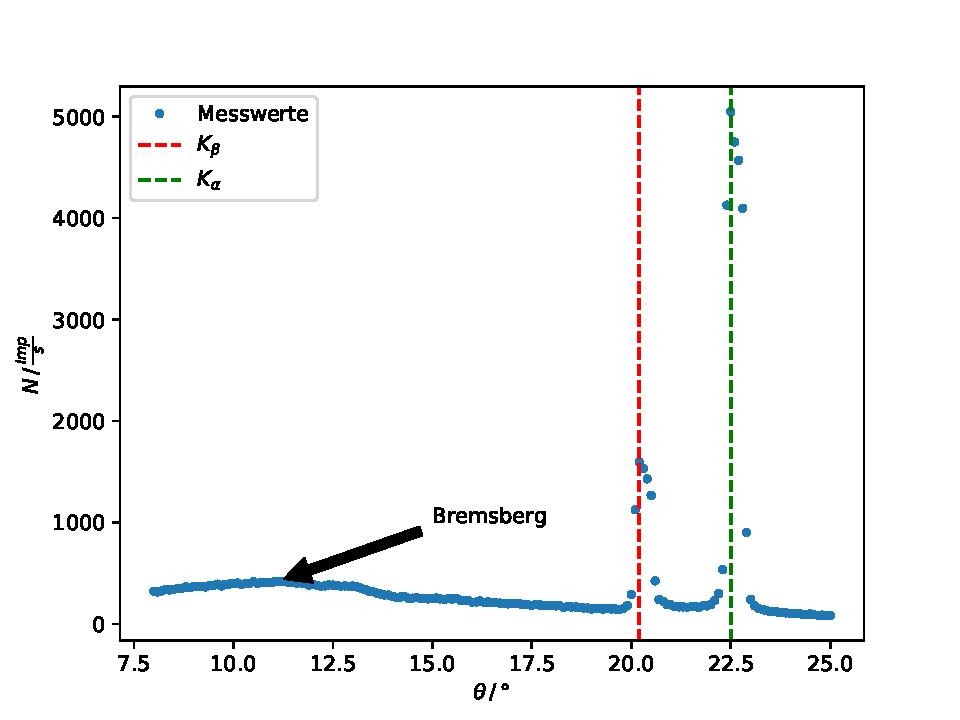
\includegraphics[width=0.7\textwidth]{content/data/plot.pdf}
    \caption{Emissionsspektrum graphisch dargestellt. \cite{numpy}}
    \label{fig:spektrum}
\end{figure}
Die Energie berechnet sich nach
\begin{equation}
    E = \frac{\symup{h}\symup{c}}{\lambda}
    \label{eqn:energie}
\end{equation}
Der erste Peak befindet sich bei $\theta, N = (20.2, 1599.0)$ und der zweite bei $\theta, N = (22.5, 5050.0)$.
Daraus folgt für die Energie \autoref{eqn:energie}
\begin{equation*}
    E_1 = \SI{1.4282e-15}{\joule}
\end{equation*}
\begin{equation*}
    E_2 = \SI{1.2887e-15}{\joule}
\end{equation*}
, wobei $\lambda$ aus \autoref{eqn:lambdaalpha} folgt.
Der Literaturwert für die $K_\alpha$-Linie \cite{klinie} beträgt
\begin{equation*}
    E_\alpha = \SI{1.2914e-15}{\joule}
\end{equation*}
und für die $K_\beta$-Linie \cite{klinie}
\begin{equation*}
     E_\beta = \SI{1.4291e-15}{\joule} .
\end{equation*}
%Aufgabe 2.1
\subsection{Bestimmung der Transmission}
\label{sec:transmission}
Die Zählrate wird in $\Delta\alpha=\SI{0.1}{\degree}$-Schritten mit Aluminum-Absorber $N_\text{Al}$ und ohne $N_0$ gemessen.
Die Messwerte sind in Tab. \ref{tab:al} aufgeführt.
Es wurde eine Integrationszeit von $t=\SI{200}{\second}$ verwendet.
Die Messunsicherheit berechnet sich nach
\begin{equation}
    \Delta N=\frac{\sqrt{N \cdot t}}{t} .
\end{equation}
Für die folgenden Fehlerrechnungen wird das Plugin uncertainties \cite{uncertainties} verwendet.
Die Wellenlänge $\lambda$ ergibt sich sofort aus dem Winkel $\theta$ (\autoref{eqn:lambdaalpha}).
Nach Beachtung der Totzeit des Geiger-Müller-Zählrohrs von $t=\SI{90}{\micro\second}$, ergeben sich die korrigierten Zählraten $I_\text{Al}$, $I_0$ \ref{eqn:totzeit}.
Die Transmission berechnet sich nach
\begin{equation*}
    T = \frac{I_\text{Al}}{I_0} .
\end{equation*}
\\
Mithilfe einer linearen Ausgleichsrechnung
\begin{equation}
    T = a \cdot \lambda + b
    \label{eqn:gerade}
\end{equation}
ergeben sich folgende Parameter:
\begin{equation*}
    a = \SI{-1.461(25)e10}{\frac{1}{\metre}}
\end{equation*}
\begin{equation*}
    b = \SI{1.189(16)}{}
\end{equation*}
Die Messdaten und die Ausgleichsgerade sind in der Abb. \ref{fig:trans} dargestellt.
\begin{figure}
    \centering
    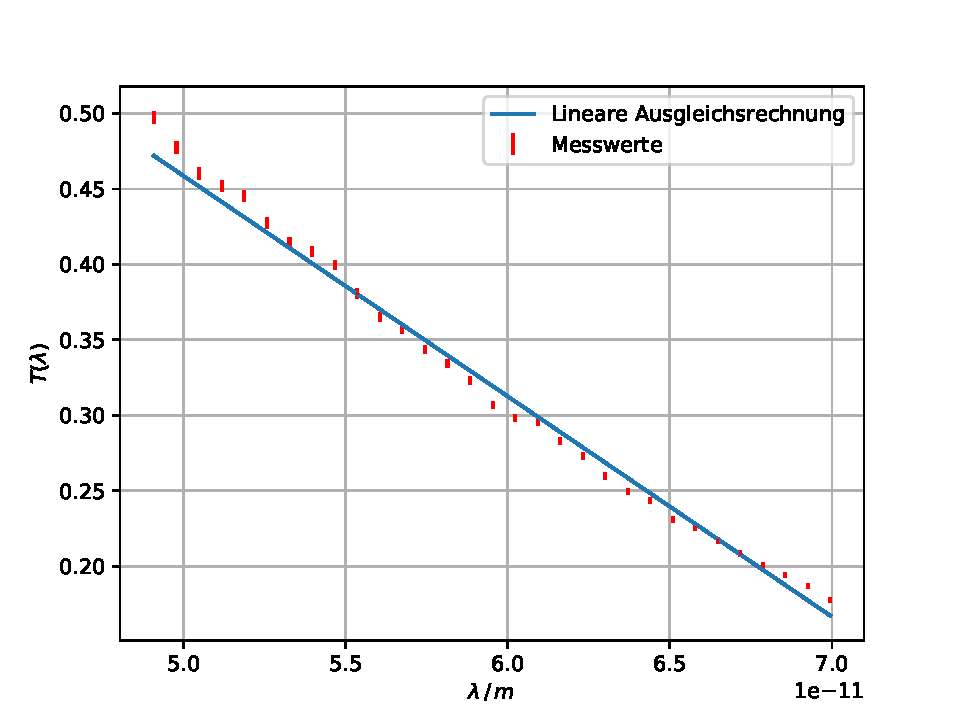
\includegraphics[width=0.7\textwidth]{content/data/linear.pdf}
    \caption{Messdaten und lineare Ausgleichsrechnung für $T(\lambda)$. \cite{matplotlib} \cite{scipy}}
    \label{fig:trans}
\end{figure}

%Aufgabe 2.2
\subsection{Bestimmung der Compton-Wellenlänge}
\label{sec:compton}
Die folgenden Zählraten wurden gemessen:
\begin{equation*}
    I_0 = \SI{2731}{\text{Impulse}}
\end{equation*}
\begin{equation*}
    I_1 = \SI{1180}{\text{Impulse}}
\end{equation*}
\begin{equation*}
    I_2 = \SI{1024}{\text{Impulse}}
\end{equation*}
Dabei wurde $I_0$ ohne Absorber, $I_1$ mit Absorber zwischen Röntgenröhre und Streuer und $I_2$ mit Absorber zwischen Streuer und Geiger-Müller-Zählrohr gemessen.
Die Transmissionen ergeben sich direkt aus den Verhältnissen
\begin{equation*}
    T_1 = \frac{I_1}{I_0} = \frac{1180}{2731}
\end{equation*}
und
\begin{equation*}
    T_2 = \frac{I_2}{I_0} = \frac{1024}{2731} .
\end{equation*}
Nun wird die lineare Gleichung \ref{eqn:gerade} nach $\lambda$ umgestellt
\begin{equation}
    \lambda = \frac{T - b}{a}
\end{equation}
und die Transmissionen eingesetzt um die jeweiligen Wellenlängen zu bestimmen:
\begin{equation*}
    \lambda_1 = \SI{5.18(14)e-11}{\metre}
\end{equation*}
\begin{equation*}
    \lambda_2 = \SI{5.57(14)e-11}{\metre}
\end{equation*}
Die Compton-Wellenlänge $\lambda_c$ folgt nun aus der Differenz der Wellenlängen $\lambda_1$ und $\lambda_2$
\begin{equation}
    \lambda_\text{c} = \SI{3.91(7)e-12}{\metre} .
    \label{eqn:lambdac}
\end{equation}